

\subsection{In-Depth Analysis of \sysp}

\begin{figure}[t]
    \centering
    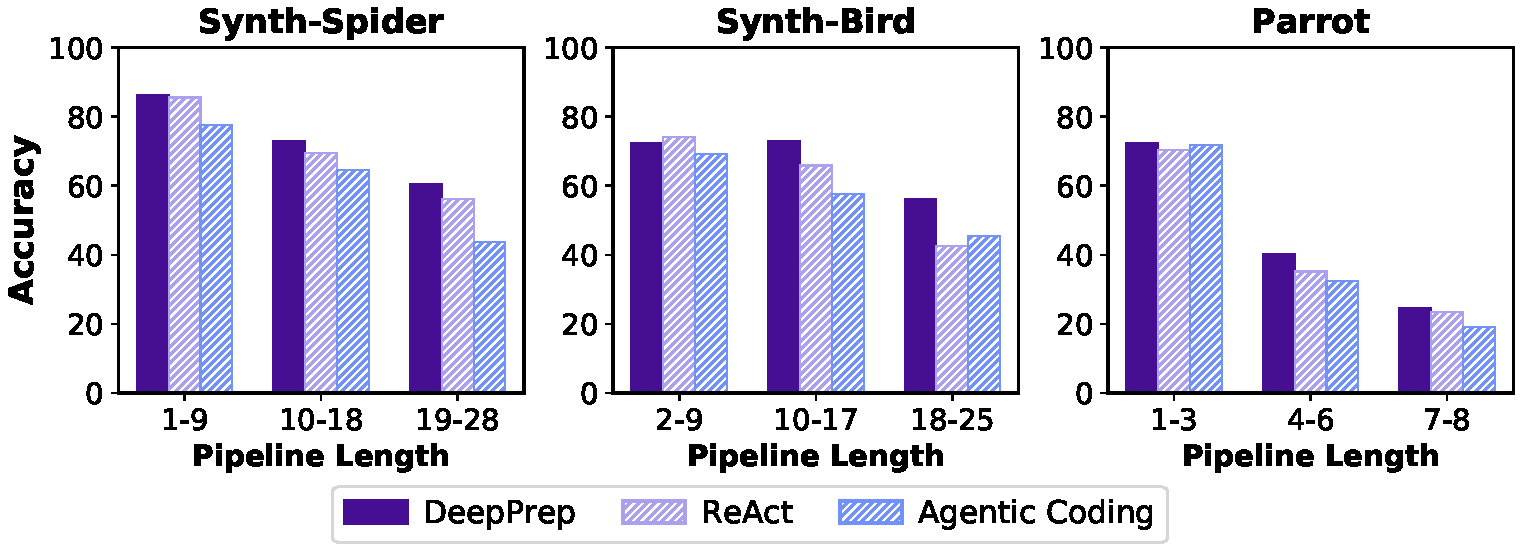
\includegraphics[width=1.01\columnwidth]{plots/plot/performance_compare_on_task_diff_claude.pdf}
    \vspace{-2em} 
    \caption{Comparison on Accuracy with varying Pipeline Length.}
    \label{\labelprefix fig:performance_compare_on_task_diff_claude}
    \vspace{-1em}
\end{figure}

% \begin{figure}[t]
    \centering
    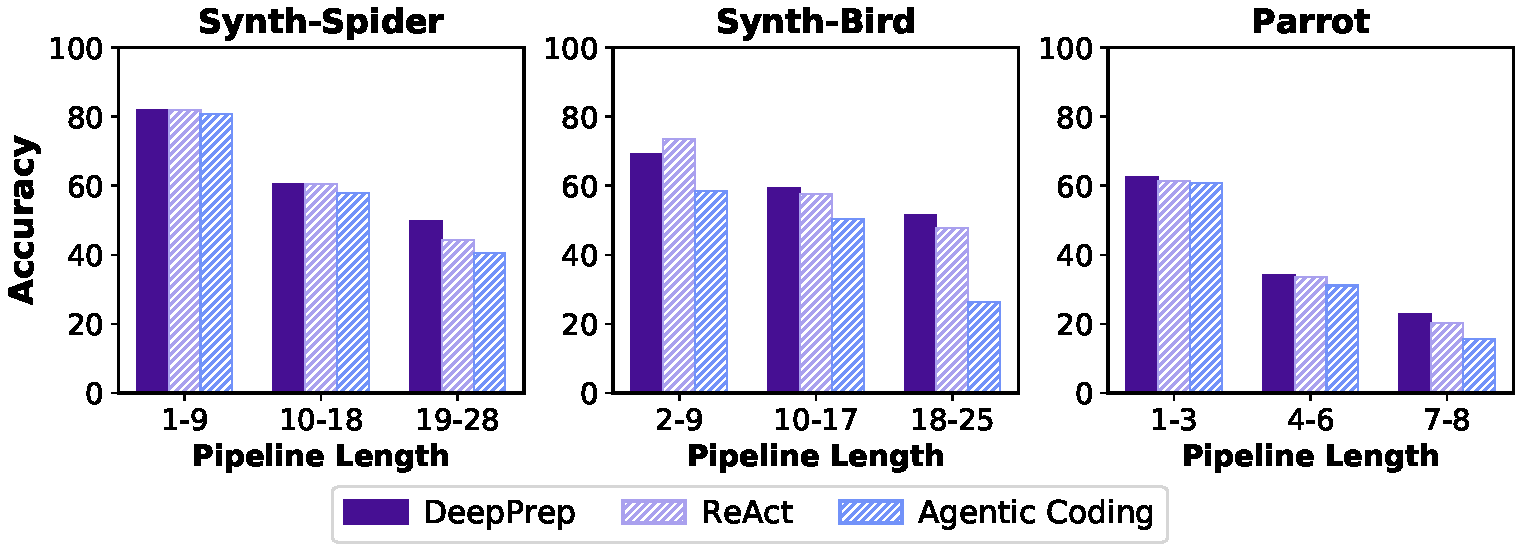
\includegraphics[width=1.01\columnwidth]{plots/plot/performance_compare_on_task_diff_r1.pdf}
    \vspace{-1em} 
    \caption{Performance Compare of different methods based on DeepSeek-R1 on cases with various difficulty.}
    \label{fig:performance_compare_on_task_diff_r1}
    \vspace{-1em}
\end{figure}

% \noindent \textbf{Exp-\expnum\label{exp:evaluate_on_various_diff}: Evaluation of \sysp on cases with different difficulty.}

\noindent \textbf{Exp-\expnum\label{exp:evaluate_on_various_diff}: Evaluation of \sysp on cases with different difficulty.}
We further analyze the performance of \sysp under different difficulty levels. Specifically, we sort all cases based on the length of their ground-truth operator pipelines and divide into three equal subsets (\textit{Simple}, \textit{Medium}, and \textit{Complex}).
We report the results of \sysp compared with three strong baselines with the Claude backbone in Figure~\ref{fig:performance_compare_on_task_diff_claude}.

As shown in Figure~\ref{fig:performance_compare_on_task_diff_claude}, \sysp exhibits superior resilience on \textbf{complex} tasks.
On {Simple} cases, the performance gap is relatively narrow; for instance, on DP-Bird (Simple), ReAct performs comparably to \sysp, indicating that linear reasoning suffices for short-horizon tasks.
However, on {Complex} tasks involving long-horizon operations, \sysp significantly outperforms baselines. 
Notably, on the {DP-Bird (Complex)} subset, \sysp maintains a robust accuracy of {56.29\%}, surpassing ReAct and MCTS-OP by a substantial margin of over \textbf{13\%}. 
The main reason is that linear approaches (like ReAct and AgenticCoding) suffer from severe error accumulation in long sequences. In contrast, \sysp utilizes a tree-based search strategy that allows for backtracking when logical inconsistencies arise, effectively mitigating the error cascading effect in complex data preparation workflows.

\begin{shaded}
\noindent \textbf{Finding \findingnum: While baselines remain competitive on simple tasks, \sysp dominates in complex DP scenarios.}
\end{shaded}

\begin{figure}[t]
    \centering
    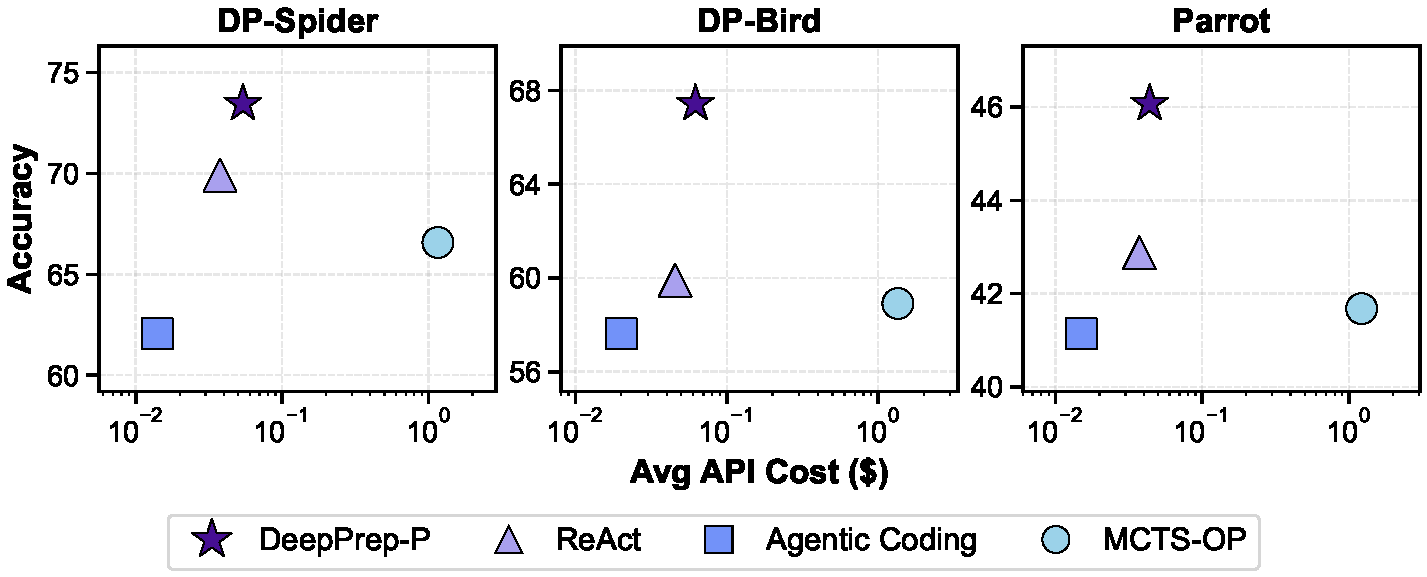
\includegraphics[width=0.99\columnwidth]{plots/plot/acc_cost_tradeoff_claude.pdf}
    \vspace{-1em} 
    \caption{Comparison of \sys and baselines based on Claude-4 on Accuracy and API cost.}
    \label{fig:acc_cost_tradeoff_claude}
  \vspace{-0.5em}
\end{figure}
% \begin{figure}[t]
    \centering
    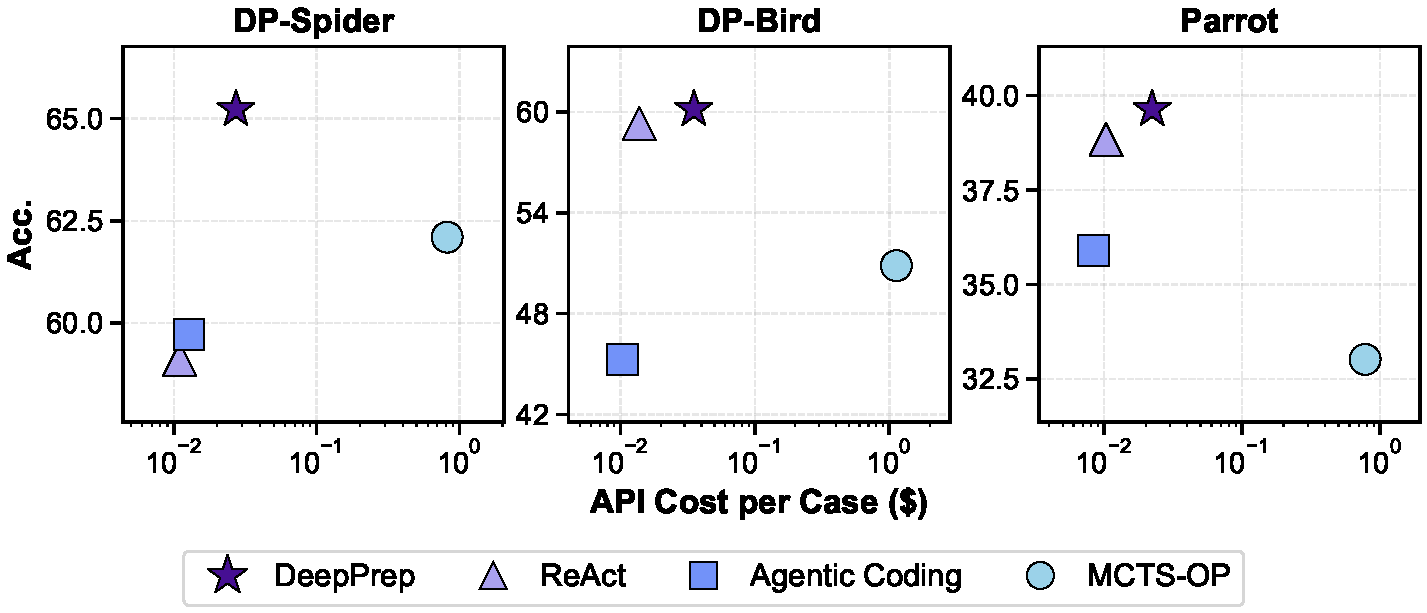
\includegraphics[width=0.99\columnwidth]{plots/plot/acc_cost_tradeoff_r1.pdf}
    \vspace{-1em} 
    \caption{Trade-off between Accuracy and API cost.}
    \label{fig:acc_cost_tradeoff_r1}
    \vspace{-1em}
\end{figure}
% \begin{figure}[t]
    \centering
    % --- 第一个子图 (Claude) ---
    \begin{subfigure}[b]{0.99\columnwidth}
        \centering
        % width=\linewidth 让图片充满子图的宽度
        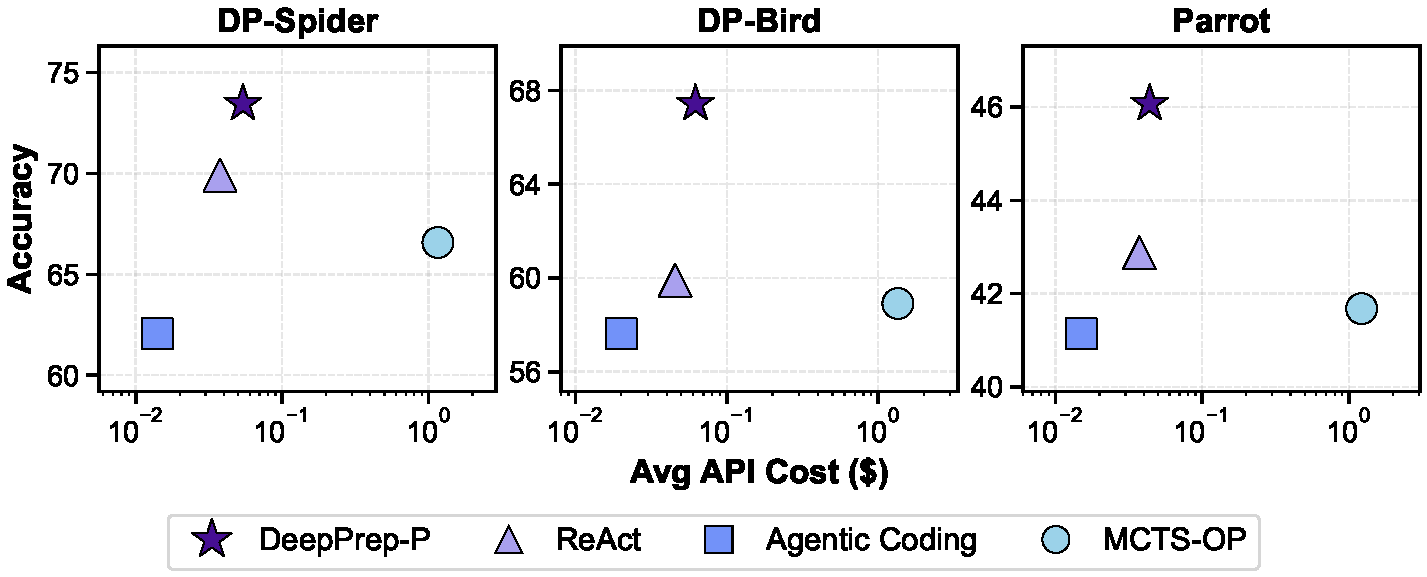
\includegraphics[width=\linewidth]{plots/plot/acc_cost_tradeoff_claude.pdf}
        \caption{Claude} % 这里写该子图对应的 LLM 名称
        \label{fig:acc_cost_tradeoff_claude}
    \end{subfigure}
    
    \vspace{1em} % 调整两个子图之间的垂直间距
    
    % --- 第二个子图 (R1) ---
    \begin{subfigure}[b]{0.99\columnwidth}
        \centering
        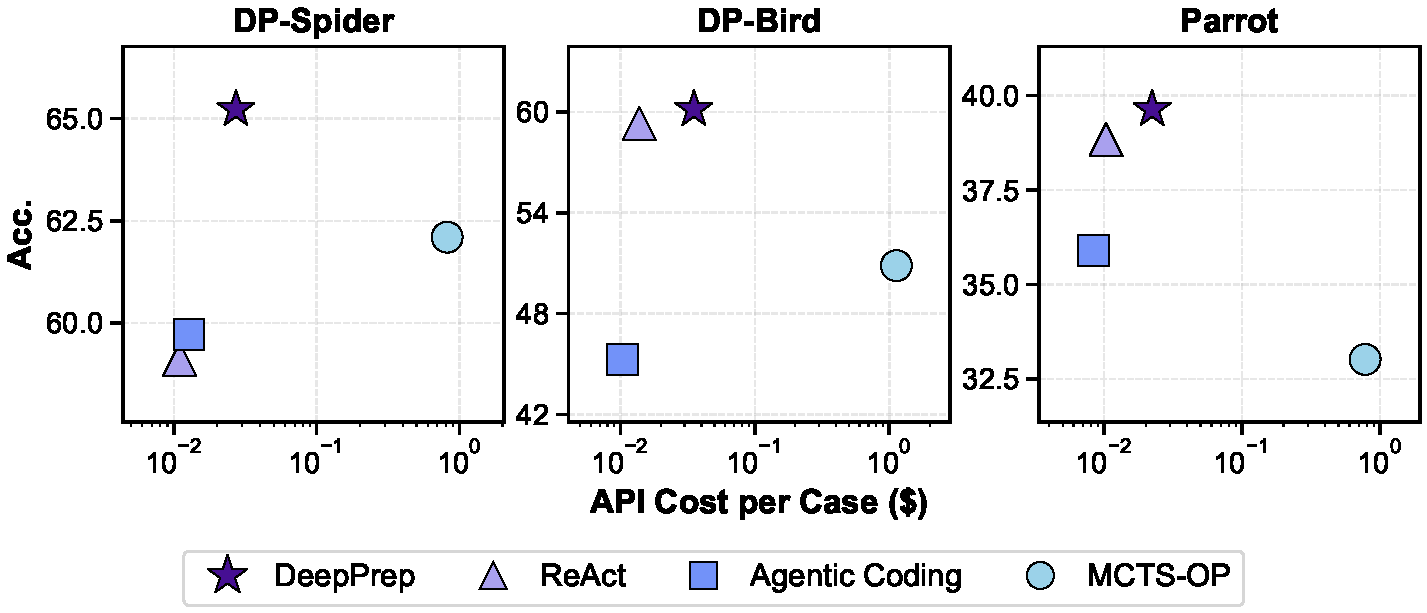
\includegraphics[width=\linewidth]{plots/plot/acc_cost_tradeoff_r1.pdf}
        \caption{R1} % 这里写该子图对应的 LLM 名称
        \label{fig:acc_cost_tradeoff_r1}
    \end{subfigure}
    
    \vspace{-0.5em} 
    % 总标题
    \caption{Trade-off between Accuracy and API cost. We compare the performance on (a) Claude and (b) R1.}
    \label{fig:acc_cost_tradeoff_combined}
    \vspace{-1em}
\end{figure}


\noindent \textbf{Exp-\expnum\label{exp:acc_cost_tradeoff}: Analysis of the trade-off between accuracy and API cost.}
We further analyze the trade-off between performance and inference cost, where the ideal method should reside in the top-left region (high accuracy, low cost).
As illustrated in Figure~\ref{fig:acc_cost_tradeoff_claude}, \sysp achieves the optimal cost-performance ratio among all methods.
Specifically ,while MCTS-OP incurs prohibitive costs (e.g., \textbf{\$1.35} per case on DP-Bird) due to extensive rollout sampling, \sysp achieves significantly higher accuracy (\textbf{67.43\%} vs. 58.91\%) with cost of \textbf{\$0.062}. This represents a cost reduction of over \textbf{21$\times$}, attributed to our efficient agentic pruning strategy which avoids brute-force search. 
Furthermore, compared to linear baselines like ReAct, \sysp incurs only a marginal cost increase (e.g., $\sim$\$0.016 difference on DP-Bird) but achieves substantial performance gains (\textbf{+6.72\%}). 
The additional computational investment in \sysp yields a high return in terms of correctness, making it the most practical choice for real-world applications.

\begin{shaded}
\noindent \textbf{Finding \findingnum: \sysp achieves the best cost-performance ratio, with the highest accuracy and a reduction of inference costs by $\sim$21$\times$ compared to MCTS-OP method.}
\end{shaded}

\begin{figure}[t]
    \centering
    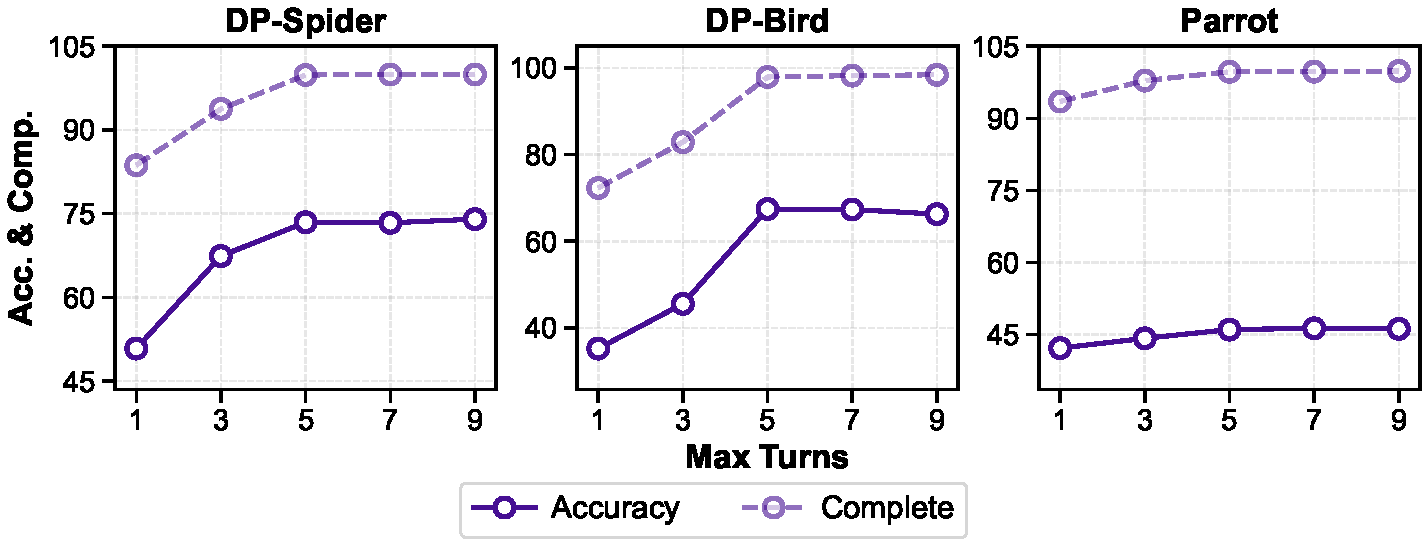
\includegraphics[width=0.99\columnwidth]{plots/plot/performance_vary_maxturn.pdf}
    \vspace{-1em} 
    \caption{Performance when changing the exploration turn.}
    \label{fig:performance_vary_maxturn}
  \vspace{-0.5em}
\end{figure}

\noindent \textbf{Exp-\expnum\label{exp:turn_number_influence}: Impact of Maximum Exploration Turns.}
We investigate how the maximum number of exploration turns affects the performance of \sysp. Figure~\ref{fig:performance_vary_maxturn} illustrates that both Accuracy and Completion Rate improve as the turns increase from 1 to 5.
Specifically, the Accuracy achieves a growth over \textbf{32\%} on DP-Bird and \textbf{22\%} on DP-Spider, while the Completion Rate steadily rises and keep around \textbf{98\%-99\%} across all datasets.
Beyond 5 turns, both metrics tend to stabilize, indicating that the model is capable of finding the optimal and executable solution within this range.
Therefore, we select 5 as the default setting to balance efficiency and effectiveness.

\begin{shaded}
\noindent \textbf{Finding \findingnum: The growth of \sysp's performance slows down after 5 exploration turns.}
\end{shaded}